% ----------------------------------------------------------
% Anexo A
% ----------------------------------------------------------
\chapter*{Anexo A - Esquema Entidade-Relacionamento (ER) e DBML}
\addcontentsline{toc}{chapter}{Anexo A - Esquema Entidade-Relacionamento (ER) e DBML}
\label{anexo:er-dbml}

Este anexo descreve a estrutura do banco de dados relacional proposto para o sistema VOEBEM, mostrando as entidades principais, seus atributos e os relacionamentos entre elas.

\section*{Diagrama ER}

\begin{figure}[htbp]
    \centering
    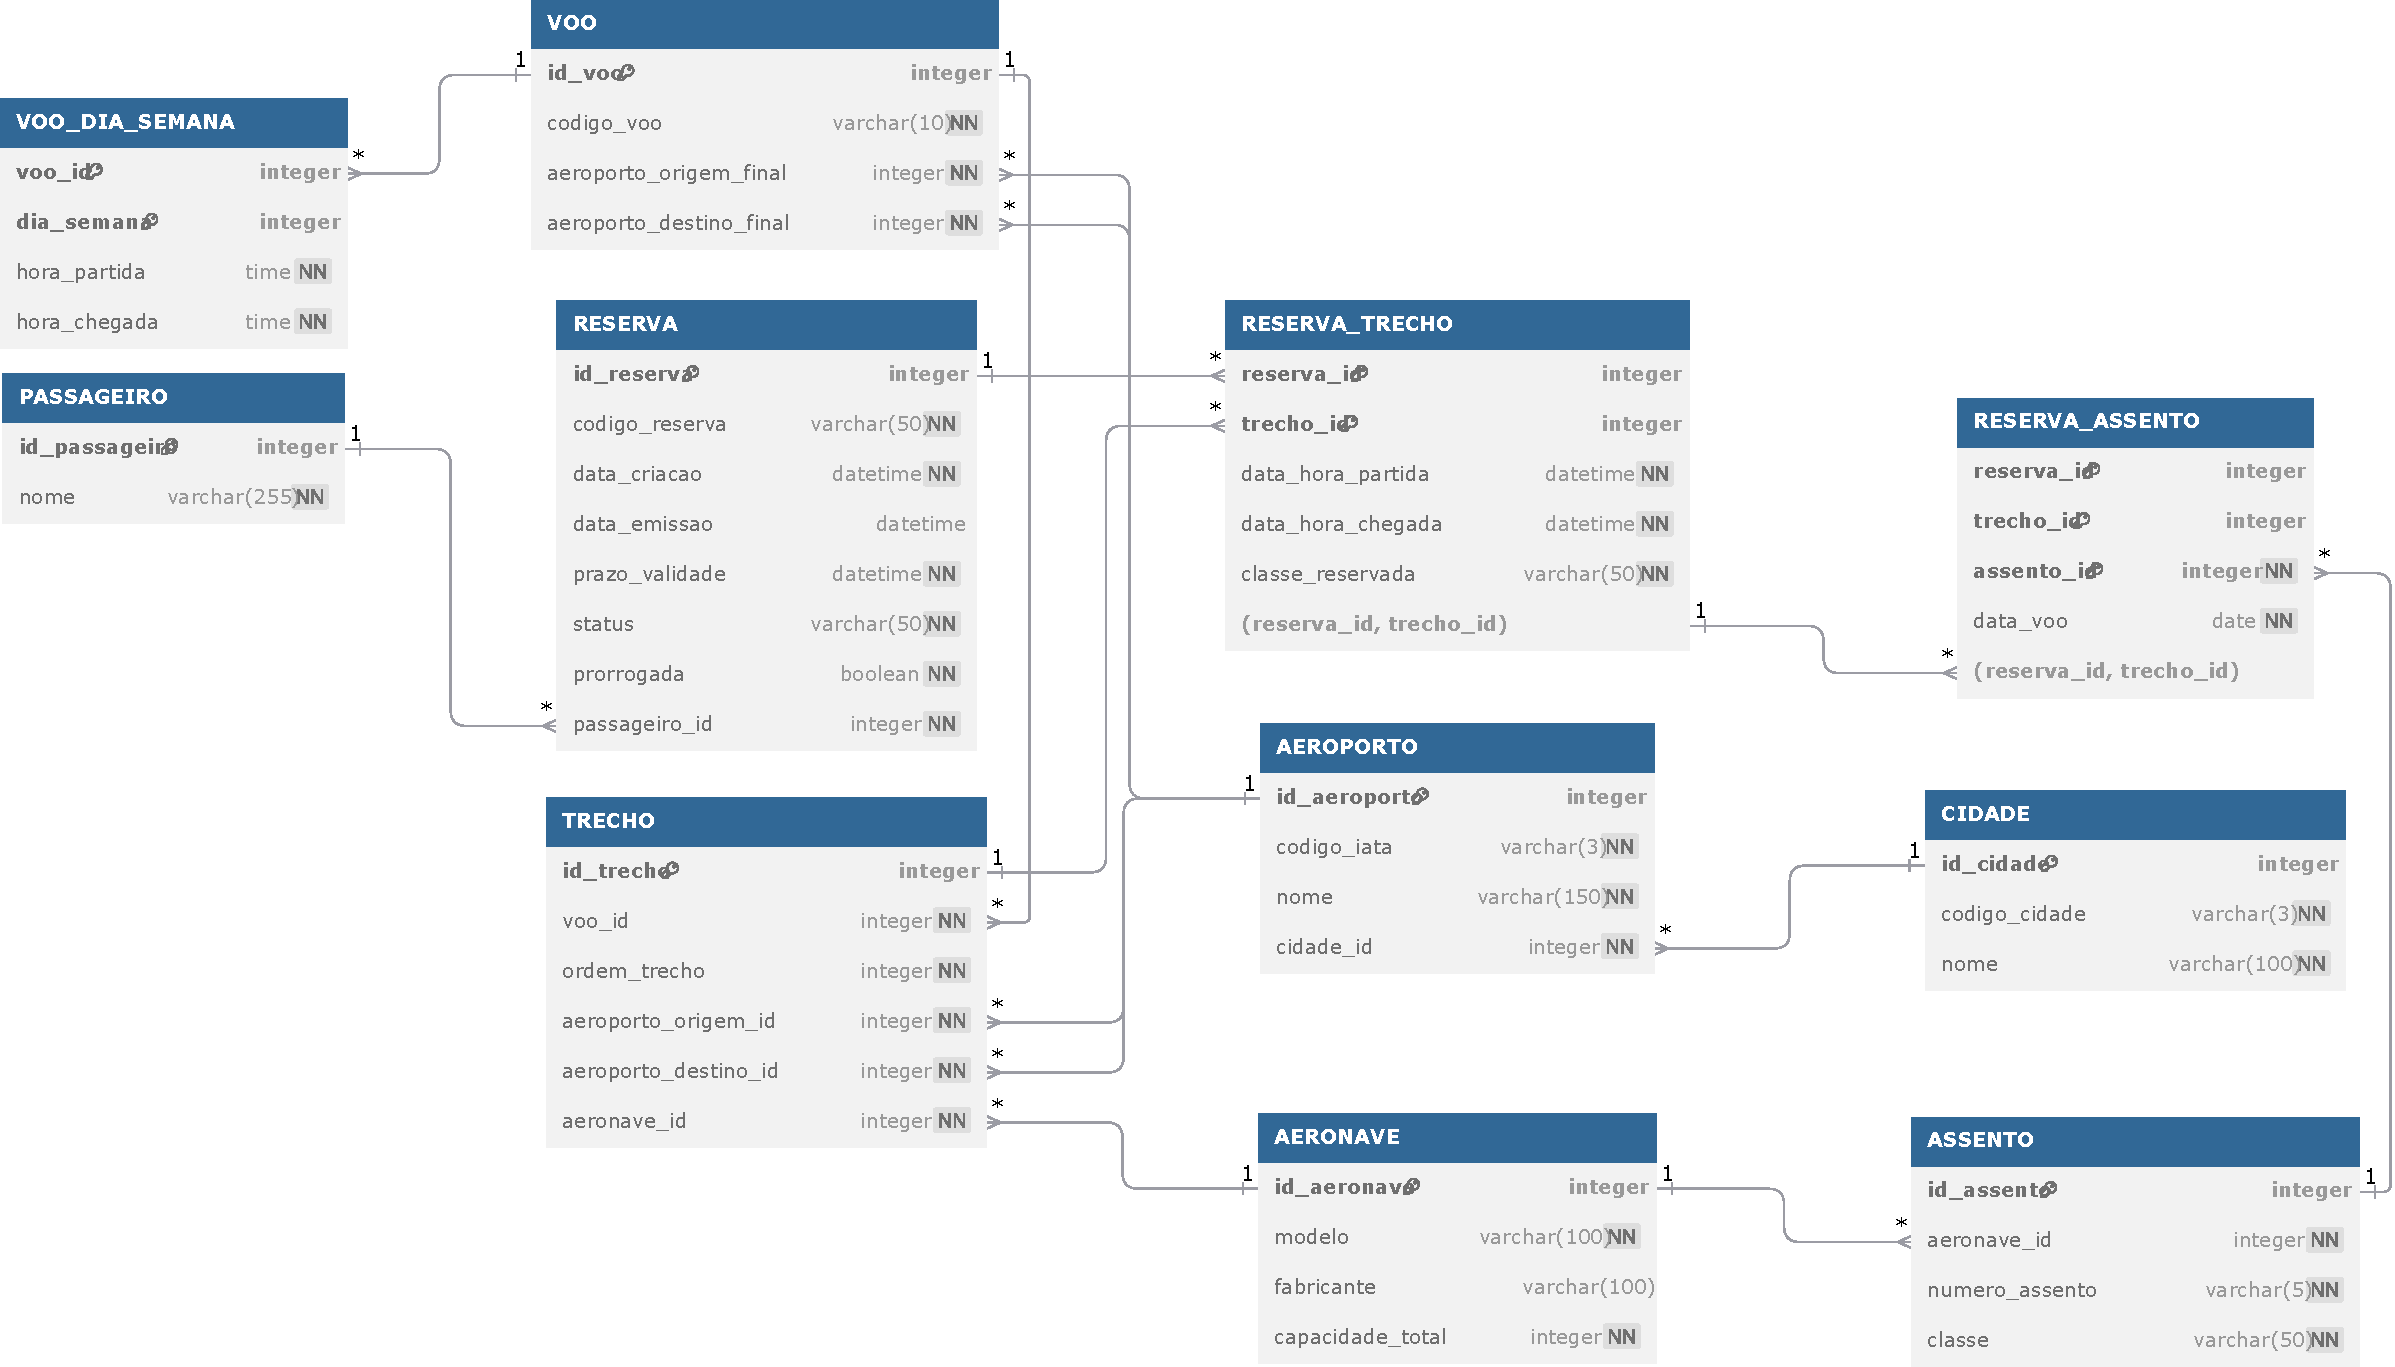
\includegraphics[width=1.4\textwidth, angle=90]{../assets/er-diagram-voebem.pdf}
    \caption{Diagrama ER - Sistema VOEBEM}
    \label{fig:diagrama-er}
\end{figure}

\textit{(Nota: O diagrama acima representa visualmente o esquema definido abaixo.)}

\section*{Descrição das Entidades e Relacionamentos}

\subsection*{Entidades}

\subsubsection*{PASSAGEIRO}
Representa uma pessoa que faz uma reserva.
\begin{itemize}
    \item \texttt{id\_passageiro} (INTEGER): Chave primária, auto-incremento.
    \item \texttt{nome} (VARCHAR): Nome do passageiro, não nulo.
\end{itemize}

\subsubsection*{RESERVA}
Representa uma reserva feita por um passageiro para um ou mais trechos de voo.
\begin{itemize}
    \item \texttt{id\_reserva} (INTEGER): Chave primária, auto-incremento.
    \item \texttt{codigo\_reserva} (VARCHAR): Código único da reserva, não nulo.
    \item \texttt{data\_criacao} (DATETIME): Data e hora de criação da reserva, não nulo (padrão: data/hora atual).
    \item \texttt{data\_emissao} (DATETIME): Data e hora de emissão (confirmação) da reserva, pode ser nulo.
    \item \texttt{prazo\_validade} (DATETIME): Prazo limite para confirmação da reserva, não nulo.
    \item \texttt{status} (VARCHAR): Status atual da reserva (Ex: Pendente, Confirmada, Cancelada, Emitida), não nulo.
    \item \texttt{prorrogada} (BOOLEAN): Indica se o prazo de validade foi prorrogado, não nulo (padrão: false).
    \item \texttt{passageiro\_id} (INTEGER): Chave estrangeira referenciando o passageiro que fez a reserva, não nulo.
    \item \texttt{fonte\_reserva} (VARCHAR): Origem da reserva (Ex: Interno, Web, GDS\_Amadeus), pode ser nulo.
    \item \texttt{id\_externo\_reserva} (VARCHAR): ID da reserva no sistema externo (Ex: GDS PNR), pode ser nulo.
    \item \texttt{id\_transacao\_pagamento} (VARCHAR): ID da transação no sistema de pagamento, pode ser nulo.
    \item \texttt{status\_pagamento} (VARCHAR): Status do pagamento (Ex: Pendente, Aprovado, Falhou), pode ser nulo.
    \item \texttt{valor\_pago} (DECIMAL): Valor efetivamente pago pela reserva, pode ser nulo.
\end{itemize}

\subsubsection*{VOO}
Representa um voo como uma sequência de trechos, com origem e destino finais.
\begin{itemize}
    \item \texttt{id\_voo} (INTEGER): Chave primária, auto-incremento.
    \item \texttt{codigo\_voo} (VARCHAR): Código único do voo, não nulo.
    \item \texttt{aeroporto\_origem\_final} (INTEGER): Chave estrangeira referenciando o aeroporto de origem final do voo, não nulo.
    \item \texttt{aeroporto\_destino\_final} (INTEGER): Chave estrangeira referenciando o aeroporto de destino final do voo, não nulo.
\end{itemize}

\subsubsection*{TRECHO}
Representa um segmento individual de um voo, conectando dois aeroportos com uma aeronave específica.
\begin{itemize}
    \item \texttt{id\_trecho} (INTEGER): Chave primária, auto-incremento.
    \item \texttt{voo\_id} (INTEGER): Chave estrangeira referenciando o voo ao qual este trecho pertence, não nulo.
    \item \texttt{ordem\_trecho} (INTEGER): Ordem do trecho dentro do voo, não nulo (compõe chave única com \texttt{voo\_id}).
    \item \texttt{aeroporto\_origem\_id} (INTEGER): Chave estrangeira referenciando o aeroporto de origem deste trecho, não nulo.
    \item \texttt{aeroporto\_destino\_id} (INTEGER): Chave estrangeira referenciando o aeroporto de destino deste trecho, não nulo.
    \item \texttt{aeronave\_id} (INTEGER): Chave estrangeira referenciando a aeronave usada neste trecho, não nulo.
\end{itemize}

\subsubsection*{VOO\_DIA\_SEMANA}
Indica em quais dias da semana um voo específico opera e seus horários.
\begin{itemize}
    \item \texttt{voo\_id} (INTEGER): Chave primária composta, chave estrangeira referenciando o voo.
    \item \texttt{dia\_semana} (INTEGER): Chave primária composta, dia da semana (0=Domingo, 6=Sábado).
    \item \texttt{hora\_partida} (TIME): Hora de partida neste dia da semana, não nulo.
    \item \texttt{hora\_chegada} (TIME): Hora de chegada neste dia da semana, não nulo.
\end{itemize}

\subsubsection*{CIDADE}
Representa uma cidade.
\begin{itemize}
    \item \texttt{id\_cidade} (INTEGER): Chave primária, auto-incremento.
    \item \texttt{codigo\_cidade} (VARCHAR): Código único da cidade (Ex: SAO), não nulo.
    \item \texttt{nome} (VARCHAR): Nome da cidade, não nulo.
\end{itemize}

\subsubsection*{AEROPORTO}
Representa um aeroporto.
\begin{itemize}
    \item \texttt{id\_aeroporto} (INTEGER): Chave primária, auto-incremento.
    \item \texttt{codigo\_iata} (VARCHAR): Código IATA único do aeroporto (Ex: GRU), não nulo.
    \item \texttt{nome} (VARCHAR): Nome do aeroporto, não nulo.
    \item \texttt{cidade\_id} (INTEGER): Chave estrangeira referenciando a cidade onde o aeroporto está localizado, não nulo.
\end{itemize}

\subsubsection*{AERONAVE}
Representa uma aeronave.
\begin{itemize}
    \item \texttt{id\_aeronave} (INTEGER): Chave primária, auto-incremento.
    \item \texttt{modelo} (VARCHAR): Modelo da aeronave, não nulo.
    \item \texttt{fabricante} (VARCHAR): Fabricante da aeronave.
    \item \texttt{capacidade\_total} (INTEGER): Capacidade total de passageiros da aeronave, não nulo.
\end{itemize}

\subsubsection*{ASSENTO}
Representa um assento individual em uma aeronave.
\begin{itemize}
    \item \texttt{id\_assento} (INTEGER): Chave primária, auto-incremento.
    \item \texttt{aeronave\_id} (INTEGER): Chave estrangeira referenciando a aeronave à qual o assento pertence, não nulo.
    \item \texttt{numero\_assento} (VARCHAR): Número/identificação do assento (compõe chave única com \texttt{aeronave\_id}), não nulo.
    \item \texttt{classe} (VARCHAR): Classe do assento (Ex: Econômica, Executiva), não nulo.
\end{itemize}

\subsubsection*{RESERVA\_TRECHO}
Tabela associativa que liga uma RESERVA a um TRECHO específico que faz parte dessa reserva.
\begin{itemize}
    \item \texttt{reserva\_id} (INTEGER): Parte da chave primária composta, chave estrangeira referenciando a RESERVA.
    \item \texttt{trecho\_id} (INTEGER): Parte da chave primária composta, chave estrangeira referenciando o TRECHO.
    \item \texttt{data\_hora\_partida} (DATETIME): Data e hora de partida programada para este trecho na reserva, não nulo.
    \item \texttt{data\_hora\_chegada} (DATETIME): Data e hora de chegada programada para este trecho na reserva, não nulo.
    \item \texttt{classe\_reservada} (VARCHAR): Classe em que o assento foi reservado para este trecho, não nulo.
\end{itemize}

\subsubsection*{RESERVA\_ASSENTO}
Tabela associativa que liga um \texttt{RESERVA\_TRECHO} a um \texttt{ASSENTO} específico reservado para uma data de voo particular.
\begin{itemize}
    \item \texttt{reserva\_id} (INTEGER): Parte da chave primária composta, chave estrangeira referenciando \texttt{RESERVA\_TRECHO}.
    \item \texttt{trecho\_id} (INTEGER): Parte da chave primária composta, chave estrangeira referenciando \texttt{RESERVA\_TRECHO}.
    \item \texttt{assento\_id} (INTEGER): Parte da chave primária composta, chave estrangeira referenciando o ASSENTO, não nulo.
    \item \texttt{data\_voo} (DATE): Data específica em que este trecho do voo está sendo reservado para este assento (compõe chave única com \texttt{assento\_id} e \texttt{trecho\_id}), não nulo.
    \item \texttt{status\_checkin} (VARCHAR): Status do check-in para este assento/trecho (Ex: Pendente, Realizado), pode ser nulo.
\end{itemize}

\subsection*{Relacionamentos}
\begin{description}
    \item[\texttt{PASSAGEIRO} -- \texttt{RESERVA}:] \texttt{PASSAGEIRO} \textbf{faz} uma ou mais (\texttt{o\{\}}) \texttt{RESERVA}s.
    \item[\texttt{RESERVA} -- \texttt{RESERVA\_TRECHO}:] \texttt{RESERVA} \textbf{contem\_trecho} um ou mais (\texttt{o\{\}}) \texttt{RESERVA\_TRECHO}s.
    \item[\texttt{TRECHO} -- \texttt{RESERVA\_TRECHO}:] \texttt{TRECHO} \textbf{eh\_reservado\_em} zero ou mais (\texttt{o\{\}}) \texttt{RESERVA\_TRECHO}s.
    \item[\texttt{VOO} -- \texttt{TRECHO}:] \texttt{VOO} \textbf{composto\_por} um ou mais (\texttt{o\{\}}) \texttt{TRECHO}s.
    \item[\texttt{AEROPORTO} -- \texttt{TRECHO} (Origem):] \texttt{AEROPORTO} pode ser a \textbf{origem\_de} zero ou mais (\texttt{o\{\}}) \texttt{TRECHO}s.
    \item[\texttt{AEROPORTO} -- \texttt{TRECHO} (Destino):] \texttt{AEROPORTO} pode ser o \textbf{destino\_de} zero ou mais (\texttt{o\{\}}) \texttt{TRECHO}s.
    \item[\texttt{AERONAVE} -- \texttt{TRECHO}:] \texttt{AERONAVE} é \textbf{usado\_em} zero ou mais (\texttt{o\{\}}) \texttt{TRECHO}s.
    \item[\texttt{VOO} -- \texttt{VOO\_DIA\_SEMANA}:] \texttt{VOO} \textbf{opera\_em} um ou mais (\texttt{o\{\}}) \texttt{VOO\_DIA\_SEMANA}s.
    \item[\texttt{CIDADE} -- \texttt{AEROPORTO}:] \texttt{CIDADE} é \textbf{localizado\_em} zero ou mais (\texttt{o\{\}}) \texttt{AEROPORTO}s.
    \item[\texttt{AERONAVE} -- \texttt{ASSENTO}:] \texttt{AERONAVE} \textbf{possui} um ou mais (\texttt{o\{\}}) \texttt{ASSENTO}s.
    \item[\texttt{AEROPORTO} -- \texttt{VOO} (Origem Final):] \texttt{AEROPORTO} pode ser a \textbf{origem\_final\_em} zero ou mais (\texttt{o\{\}}) \texttt{VOO}s.
    \item[\texttt{AEROPORTO} -- \texttt{VOO} (Destino Final):] \texttt{AEROPORTO} pode ser o \textbf{destino\_final\_em} zero ou mais (\texttt{o\{\}}) \texttt{VOO}s.
    \item[\texttt{RESERVA\_TRECHO} -- \texttt{RESERVA\_ASSENTO}:] \texttt{RESERVA\_TRECHO} tem um \textbf{assento\_reservado\_para} zero ou mais (\texttt{o\{\}}) \texttt{RESERVA\_ASSENTO}s.
    \item[\texttt{ASSENTO} -- \texttt{RESERVA\_ASSENTO}:] \texttt{ASSENTO} é \textbf{reservado\_em} zero ou mais (\texttt{o\{\}}) \texttt{RESERVA\_ASSENTO}s.
\end{description}

\section*{Esquema DBML}

Abaixo está o esquema do banco de dados definido usando a sintaxe DBML (Database Markup Language). Este esquema é uma representação textual do diagrama ER, facilitando a criação e manutenção do banco de dados.

\begin{lstlisting}[language={}, % Nenhuma linguagem específica definida para DBML no listings
    basicstyle=\footnotesize\ttfamily, % Fonte monoespaçada pequena
    breaklines=true, % Quebra linhas longas automaticamente
    caption={Esquema DBML - Sistema VOEBEM},
    label={lst:dbml-schema},
    showstringspaces=false, % Não mostra espaços em strings de forma especial
    tabsize=2, % Define o tamanho da tabulação
    frame=single, % Adiciona uma moldura simples
    numbers=left, % Adiciona numeração de linhas à esquerda
    numberstyle=\tiny\color{gray}, % Estilo da numeração de linhas
    % --- Correções para caracteres especiais --- 
    literate={_}{{\_}}1 % Trata underscore como texto literal
             {`}{{\texttt{\`}}}1, % Trata backtick como texto literal (usando texttt)
             % Aspas simples (') parecem ok, pois já estão escapadas nas notas
             % Maior que (>) em Refs parece ok por padrão
    % -------------------------------------------
    % Estilos opcionais (podem ser removidos se causarem problemas)
    keywordstyle=\color{blue}, 
    commentstyle=\color{green!60!black}, 
    stringstyle=\color{purple}
]
Table PASSAGEIRO {
  id_passageiro integer [pk, increment]
  nome varchar(255) [not null]
}

Table RESERVA {
  id_reserva integer [pk, increment]
  codigo_reserva varchar(50) [unique, not null]
  data_criacao datetime [default: `now()`, not null]
  data_emissao datetime [null]
  prazo_validade datetime [not null]
  status varchar(50) [not null, note: 'Pendente, Confirmada, Cancelada, Expirada']
  prorrogada boolean [default: false, not null]
  passageiro_id integer [not null]

  Indexes {
    (codigo_reserva)
  }
}

Table VOO {
  id_voo integer [pk, increment]
  codigo_voo varchar(10) [unique, not null]
  aeroporto_origem_final integer [not null]
  aeroporto_destino_final integer [not null]
  Indexes {
    (codigo_voo)
  }
}

Table TRECHO {
  id_trecho integer [pk, increment]
  voo_id integer [not null]
  ordem_trecho integer [not null, note: 'Sequência do trecho dentro do voo (1, 2, ...)' ]
  aeroporto_origem_id integer [not null]
  aeroporto_destino_id integer [not null]
  aeronave_id integer [not null, note: 'Aeronave planejada para este trecho']

  Indexes {
    (voo_id, ordem_trecho) [unique]
  }
}

Table VOO_DIA_SEMANA {
  voo_id integer [pk]
  dia_semana integer [pk, note: '0=Domingo, 1=Segunda,..., 6=Sábado']
  hora_partida time [not null]
  hora_chegada time [not null]
}

Table CIDADE {
  id_cidade integer [pk, increment]
  codigo_cidade varchar(3) [unique, not null, note: 'Ex: SAO, RIO']
  nome varchar(100) [not null]

  Indexes {
    (codigo_cidade)
  }
}

Table AEROPORTO {
  id_aeroporto integer [pk, increment]
  codigo_iata varchar(3) [unique, not null, note: 'Ex: GRU, GIG, POA']
  nome varchar(150) [not null]
  cidade_id integer [not null]

  Indexes {
    (codigo_iata)
  }
}

Table AERONAVE {
  id_aeronave integer [pk, increment]
  modelo varchar(100) [not null]
  fabricante varchar(100)
  capacidade_total integer [not null]
}

Table ASSENTO {
  id_assento integer [pk, increment]
  aeronave_id integer [not null]
  numero_assento varchar(5) [not null, note: 'Ex: 1A, 20F']
  classe varchar(50) [not null, note: 'Econômica, Executiva, Primeira Classe']

  Indexes {
    (aeronave_id, numero_assento) [unique]
  }
}

Table RESERVA_TRECHO {
  reserva_id integer [pk]
  trecho_id integer [pk]
  data_hora_partida datetime [not null, note: 'Data e hora exatas da partida deste trecho para esta reserva']
  data_hora_chegada datetime [not null, note: 'Data e hora exatas da chegada deste trecho para esta reserva']
  classe_reservada varchar(50) [not null, note: 'Classe específica reservada para este trecho (pode ser diferente da classe do assento)']
}

Table RESERVA_ASSENTO {
  reserva_id integer [pk]
  trecho_id integer [pk]
  assento_id integer [pk, not null]
  data_voo date [not null, note: 'Data específica do voo para esta reserva de assento']

  Indexes {
    (assento_id, trecho_id, data_voo) [unique]
  }
}

Ref: RESERVA.passageiro_id > PASSAGEIRO.id_passageiro
Ref: RESERVA_TRECHO.reserva_id > RESERVA.id_reserva
Ref: RESERVA_TRECHO.trecho_id > TRECHO.id_trecho
Ref: TRECHO.voo_id > VOO.id_voo
Ref: TRECHO.aeroporto_origem_id > AEROPORTO.id_aeroporto
Ref: TRECHO.aeroporto_destino_id > AEROPORTO.id_aeroporto
Ref: TRECHO.aeronave_id > AERONAVE.id_aeronave
Ref: VOO_DIA_SEMANA.voo_id > VOO.id_voo
Ref: AEROPORTO.cidade_id > CIDADE.id_cidade
Ref: ASSENTO.aeronave_id > AERONAVE.id_aeronave
Ref: VOO.aeroporto_origem_final > AEROPORTO.id_aeroporto
Ref: VOO.aeroporto_destino_final > AEROPORTO.id_aeroporto
Ref: RESERVA_ASSENTO.(reserva_id, trecho_id) > RESERVA_TRECHO.(reserva_id, trecho_id)
Ref: RESERVA_ASSENTO.assento_id > ASSENTO.id_assento
\end{lstlisting}

% --- Final do Arquivo ---